\documentclass[../../tc_tp6_main.tex]{subfiles}
\usepackage{tikzit}
\input{sample.tikzstyles}


\begin{document}
\chapter{PLL}

Un PLL es un circuito que permite generar una se\~nal de salida con la misma frecuencia que la se\~nal de entrada. Esta sincronizaci\'on se mantiene incluso con ruido en la entrada o con variaciones en la frecuencia de entrada dentro de cierto rango.

\section{Funcionamiento}

\todo[inline]{que es un pll}

\begin{figure}[H]
	\centering 
	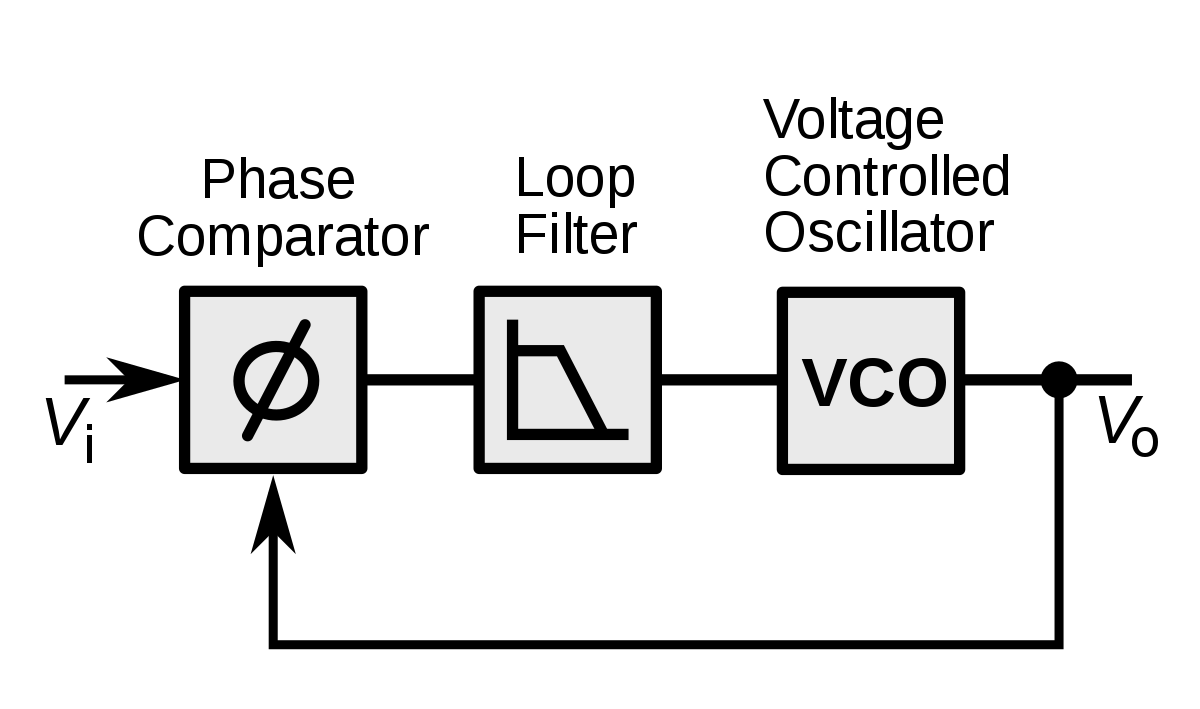
\includegraphics[width = 0.6\textwidth]{figures/pll_loop.png}
	\caption{Configuraci\'on b\'asica de un PLL}
	\label{ej2:basic_pll}
\end{figure}

\subsection{Componentes}
\subsubsection{Comparador de fase}
El comparador de fase genera una se\~nal de salida ($v_E$, o se\~nal de error) cuyo valor medio es proporcional a la diferencia de fase entre dos se\~nales de entrada. Si $K_D$ es la ganancia del detector, se obtiene la expresi\'on del valor medio de la salida:
\begin{equation}
	valor \, medio \, v_E = K_D\cdot \Delta \phi
	\label{eq:ej2_salida_comparador}
\end{equation}

Cuando las dos entradas tienen la misma frecuencia constante, la salida es tambi\'en es constante dado que $\Delta \phi$ no var\'ia. El integrado utilizado tiene dos tipos de comparadores de fase (tipo I y II), y se utiliz\'o el primero.\todo{redaccion}
\subsubsection{Tipo I}
El comparador tipo I es una compuerta XOR. El siguiente an\'alisis se realiza asumiendo que ambas entradas del comparador son se\~nales cuadradas entre 0 (low) y Vcc (high), y con duty-cycle de 50\%\todo{chequear si el vco siempre tira duty cycle de 50\%}.

Suponiendo que las entradas tienen la misma frecuencia, la salida depende unicamente de la diferencia de fase seg\'un la ecuaci\'on \ref




En la figura \ref{ej2:xor_med} se muestra el funcionamiento del comparador para dos se\~nales de frecuencia constante. En esta medici\'on no se utiliz\'o el loop de la figura \ref{ej2:basic_pll}, ya que de hacerlo, la frecuencia de la se\~nal proveniente del VCO podr\'ia variar.

\begin{figure}[H]
	\centering 
	\missingfigure{medicion comparador XOR}
	\caption{Medici\'on del comparador tipo I sin cerrar el loop.}
	\label{ej2:xor_med}
\end{figure}



\subsubsection{Tipo II}
\subsubsection{Filtro}
\subsubsection{VCO}
\subsection{Funcionamiento antes del engache}
\subsection{Funcionamiento enganchado}
\subsection{Transferencia}
\subsubsection{Sin filtro}
\subsubsection{Con filtro RC}
\subsubsection{Con filtro RRC}
\section{Aplicaciones}
\subsection{Uso como demodulador de FM}
\subsection{Uso como multiplicador de frecuencia}


\end{document}
